\documentclass[polish,envcountsect,10pt]{beamer}
    \usepackage[T1]{fontenc}
    \usepackage{polski}
    \usepackage{babel}
    \usepackage{tikz}
    \usepackage{graphicx}
    \usetheme{Warsaw}
    \title{Problem chińskiego listonosza (PCL)}
    \author{184657 Wojciech Panfil}
    \date{Gdańsk, \texorpdfstring{$9.11.2023$}{9.11.2023}}
\begin{document}

\frame{\titlepage}

\begin{frame}{Abstrakt}
    \begin{block}{Plan prezentacji}
        \begin{itemize}
            \item Część 1: Definicje.
            \item Część 2: Grafy eulerowskie, nieskierowane, nieważone.
            \item Część 3: Grafy półeulerowskie, nieskierowane, nieważone.
            \item Część 4: Grafy eulerowskie, nieskierowane, ważone.
            \item Część 5: Grafy półeulerowskie, nieskierowane, ważone.
            \item Część 6: Grafy spójne, nieeulerowskie, nieskierowane.
            \item Część 7: Zastosowania.
        \end{itemize}
    \end{block}
    \begin{block}{Omawiane algorytmy}
        \begin{itemize}
            \item Algorytm Fleury'ego
            \item Algorytm Hierholzera
            \item Algorytm ogólny
        \end{itemize}
    \end{block}
\end{frame}

\begin{frame}{Część 1 - graf eulerowski}
    \begin{block}{Graf eulerowski}
        \begin{itemize}
        \item Graf spójny mający cykl zawierający wszystkie jego krawędzie zwany cyklem Eulera.
        \item Jeżeli graf jest nieskierowany - stopień każdego wierzchołka musi być parzysty.
        \item Jeżeli graf jest skierowany - stopień wejściowy każdego wierzchołka jest równy stopniowi wyjściowemu.
        \end{itemize}
    \end{block}
    \begin{center}
        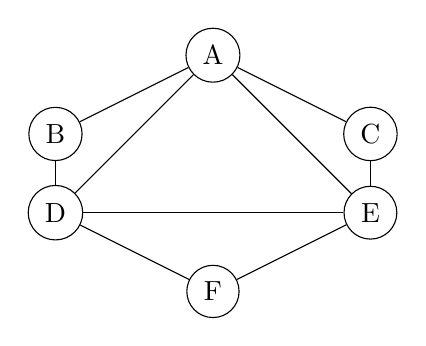
\begin{tikzpicture}
            \node[draw, circle] (A) at (0,1) {A};
            \node[draw, circle] (B) at (-2,0) {B};
            \node[draw, circle] (C) at (2,0) {C};
            \node[draw, circle] (D) at (-2,-1) {D};
            \node[draw, circle] (E) at (2,-1) {E};
            \node[draw, circle] (F) at (0,-2) {F};

            \draw (A) -- (D);
            \draw (A) -- (B);
            \draw (B) -- (D);
            \draw (A) -- (C);
            \draw (C) -- (E);
            \draw (A) -- (E);
            \draw (D) -- (E);
            \draw (D) -- (F);
            \draw (E) -- (F);
        \end{tikzpicture}
    \end{center}
\end{frame}

\begin{frame}{Część 1 - graf półeulerowski}
    \begin{block}{Graf półeulerowski}
        \begin{itemize}
            \item Graf spójny, w którym istnieje ścieżka (Eulera) przechodząca przez każdą krawędź dokładnie raz.
            \item Jeżeli graf jest nieskierowany - posiada dwa wierzchołki o stopniu nieparzystym.
            \item Jeżeli graf jest skierowany - posiada dwa wierzchołki, których stopeiń wejściowy jest różny od stopnia wyjściowego.
            \item Jeden z nich jest początkiem, drugi końcem ścieżki Eulera.
        \end{itemize}
    \end{block}
    \begin{center}
        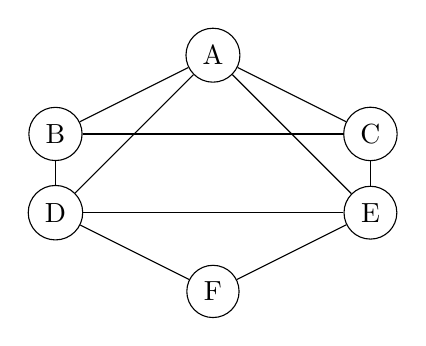
\begin{tikzpicture}
            \node[draw, circle] (A) at (0,1) {A};
            \node[draw, circle] (B) at (-2,0) {B};
            \node[draw, circle] (C) at (2,0) {C};
            \node[draw, circle] (D) at (-2,-1) {D};
            \node[draw, circle] (E) at (2,-1) {E};
            \node[draw, circle] (F) at (0,-2) {F};

            \draw (A) -- (D);
            \draw (A) -- (B);
            \draw (B) -- (D);
            \draw (A) -- (C);
            \draw (C) -- (E);
            \draw (B) -- (C);
            \draw (A) -- (E);
            \draw (D) -- (E);
            \draw (D) -- (F);
            \draw (E) -- (F);
        \end{tikzpicture}
    \end{center}
\end{frame}

\begin{frame}{Część 1 - Twierdzenie Eulera - dowód}
\begin{block}{Twierdzenie Eulera}
    Graf spójny jest eulerowski wtedy i tylko wtedy, gdy
    stopień każdego wierzchołka jest liczbą parzystą.
\end{block}
\begin{block}{Dowód}
    Jeśli $C$ jest cyklem Eulera w $G$, to trawersujemy i usuwamy
    krawędzie w $E$($G$) zgodnie z kolejnością zadaną przez $C$. Gdy przechodzimy
    przez dowolny wierzchołek $v$, to usuwamy dwie incydentne z nim krawędzie,
    więc stopień tego wierzchołka w tak zredukowanym grafie pozostaje
    parzysty.
\end{block}
\begin{figure}
    \centering
    \includegraphics[width=0.7\linewidth]{./zal_b.png}
\end{figure}
\end{frame}

\begin{frame}{Część 1 - grafy eulerowskie - historia}
    \begin{block}{Mosty królewieckie}
        Nazwa „eulerowski” pochodzi stąd, iż Euler w 1736r. rozwiązał „problem
        mostów królewieckich”. Pytano, czy można przejść dokładnie raz przez
        każdy z siedmiu mostów tak, aby powrócić do punktu wyjścia.
    \end{block}
    \begin{figure}
        \centering
        \includegraphics[width=0.7\linewidth]{./zal_a.png}
    \end{figure}
\end{frame}

\begin{frame}{Część 1 - Problem Chińskiego Listonosza}
    \begin{block}{Problem Chińskiego Listonosza}
        Celem problemu jest znalezienie ścieżki zamkniętej o minimalnej sumie wag przechodzącej przez wszystkie krawędzie co najmniej raz.
    \end{block}
    \begin{block}{Podział ze względu na rodzaj grafu}
        \begin{itemize}
            \item Graf eulerowski - przejście przez każdą krawędź jeden raz i powrót do początku.
            \item Graf półeulerowski - przejście przez każdą krawędź jeden raz.
            \item Graf (nie)ważony - cykl o minimalnej sumie wag.
            \item Graf (nie)skierowany - "ulice jednokierunkowe".
        \end{itemize}
    \end{block}
    \begin{block}{Inne, przykładowe warianty}
        \begin{itemize}
            \item Windy Chinese Postman Problem - graf ważony, koszt zależy od kierunku poruszania się.
            \item Mixed Chinese Postman Problem - graf częściowo skierowany - nie wszystkie krawędzie mają kierunek.
        \end{itemize}
    \end{block}
\end{frame}

\begin{frame}{Część 1 - historia}
    \begin{block}{Historia CPP}
        \begin{itemize}
            \item Problem Chińskiego Listonosza został wprowadzony w matematyce i teorii grafów przez chińskiego matematyka Kuan Xun w 1962 roku.
            \item Pierwsze prace nad problemem były głównie związane z rozwiązywaniem go w grafach nieskierowanych.
            \item W późniejszych latach pojawiły się badania nad wariantem problemu w grafach skierowanych.
        \end{itemize}
    \end{block}
\end{frame}

\begin{frame}{Część 2 - Algorytm Fleury'ego}
    \begin{block}{}
        \begin{itemize}
            \item Algorytm Fleury'ego służy do znajdowania cyklu lub ścieżki Eulera w spójnym grafie nieskierowanym.
            \item Algorytm ten został nazwany na cześć szwajcarskiego matematyka Gustava Fleury'ego, który opublikował go w 1883 roku.
            \item Złożoność z wyszukiwaniem mostów Tarjana ($\mathcal{O}(|E|^2)$)
        \end{itemize}
    \end{block}
\end{frame}

\begin{frame}{Część 2 - Działanie Algorytmu Fleury'ego}
    \begin{enumerate}
        \item Rozpocznij od dowolnego wierzchołka grafu. Dodaj go na stos.
        \item Wybierz dowolną krawędź wychodzącą z bieżącego wierzchołka (o ile nie jest to most)  i usuń ją z grafu.
        \item Jeżeli został wyłącznie most, wybierz go i usuń go z grafu.
        \item Przejdź do wierzchołka, do którego prowadzi wybrana, usunięta krawędź. Dodaj go na stos.
        \item Powtarzaj kroki 2-4, aż nie będzie już dostępnych krawędzi wychodzących z bieżącego wierzchołka.
        \item Algorytm kończy się, gdy wszystkie krawędzie zostaną odwiedzone i dodane do ścieżki.
    \end{enumerate}
\end{frame}

\begin{frame}{Część 2 - Algorytm Fleury'ego: przykład}
    \begin{block}{Przykład}
          Rozważmy poniższy nieważony, nieskierowany graf eulerowski.
    \end{block}
    \begin{center}
        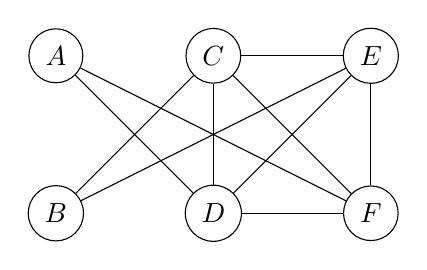
\begin{tikzpicture}
            \node[draw, circle] (A) at (0,0) {$A$};
            \node[draw, circle] (B) at (0,-2) {$B$};
            \node[draw, circle] (C) at (2,0) {$C$};
            \node[draw, circle] (D) at (2,-2) {$D$};
            \node[draw, circle] (E) at (4,0) {$E$};
            \node[draw, circle] (F) at (4,-2) {$F$};

            \draw (A) -- (D);
            \draw (A) -- (F);
            \draw (B) -- (C);
            \draw (B) -- (E);
            \draw (C) -- (D);
            \draw (C) -- (F);
            \draw (D) -- (E);
            \draw (E) -- (F);
            \draw (C) -- (E);
            \draw (F) -- (D);
        \end{tikzpicture}
    \end{center}
\end{frame}
    
\begin{frame}{Część 2 -Algorytm Fleury'ego: przykład}
    \begin{itemize}
        \item Rozpocznij od wybranego wierzchołka, na przykład wierzchołka $A$. Wpisz go na stos.
        \item Wybierz krawędź wychodzącą z wierzchołka $A$, która nie jest mostem, na przykład krawędź do $B$.
        \item Przejdź do wierzchołka $B$ i usuń krawędź z grafu.
        \item Początek został oznaczony kolorem zielonym.
        \item Obecny wierzchołek oznaczany będzie kolorem niebieskim.
        \item Stos: $A$
    \end{itemize}
    \begin{center}
        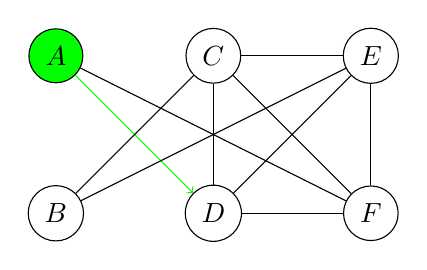
\begin{tikzpicture}
            \node[draw, circle, fill=green] (A) at (0,0) {$A$};
            \node[draw, circle] (B) at (0,-2) {$B$};
            \node[draw, circle] (C) at (2,0) {$C$};
            \node[draw, circle] (D) at (2,-2) {$D$};
            \node[draw, circle] (E) at (4,0) {$E$};
            \node[draw, circle] (F) at (4,-2) {$F$};

            \draw[->, green] (A) -- (D);
            \draw (A) -- (F);
            \draw (B) -- (C);
            \draw (B) -- (E);
            \draw (C) -- (D);
            \draw (C) -- (F);
            \draw (D) -- (E);
            \draw (E) -- (F);
            \draw (C) -- (E);
            \draw (F) -- (D);
        \end{tikzpicture}
    \end{center}
\end{frame}

\begin{frame}{Część 2 - Algorytm Fleury'ego: przykład}
    \begin{itemize}
        \item Jesteś w wierzchołku $D$. Umieść go na stosie.
        \item Wybierz krawędź wychodzącą z wierzchołka $D$, która nie jest mostem, na przykład krawędź do $C$.
        \item Przejdź do wierzchołka $C$ i usuń krawędź z grafu.
        \item Stos: $A$, $D$
    \end{itemize}
    \begin{center}
        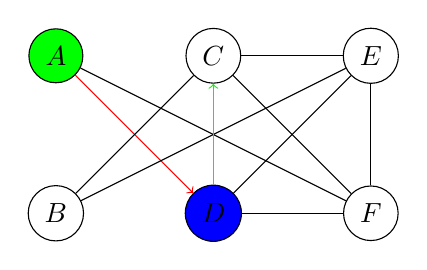
\begin{tikzpicture}
            \node[draw, circle, fill=green] (A) at (0,0) {$A$};
            \node[draw, circle] (B) at (0,-2) {$B$};
            \node[draw, circle] (C) at (2,0) {$C$};
            \node[draw, circle, fill=blue] (D) at (2,-2) {$D$};
            \node[draw, circle] (E) at (4,0) {$E$};
            \node[draw, circle] (F) at (4,-2) {$F$};

            \draw[->, red] (A) -- (D);
            \draw (A) -- (F);
            \draw (B) -- (C);
            \draw (B) -- (E);
            \draw[->, green] (D) -- (C);
            \draw (C) -- (F);
            \draw (D) -- (E);
            \draw (E) -- (F);
            \draw (C) -- (E);
            \draw (F) -- (D);
        \end{tikzpicture}
    \end{center}
\end{frame}

\begin{frame}{Część 2 - Algorytm Fleury'ego: przykład}
    \begin{itemize}
        \item Jesteś w wierzchołku $C$. Umieść go na stosie.
        \item Wybierz krawędź wychodzącą z wierzchołka $D$, która nie jest mostem, na przykład krawędź do $E$.
        \item Przejdź do wierzchołka $E$ i usuń krawędź z grafu.
        \item Stos: $A$, $D$, $C$
    \end{itemize}
    \begin{center}
        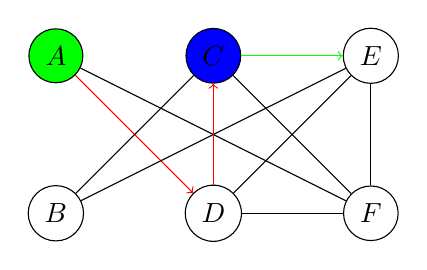
\begin{tikzpicture}
            \node[draw, circle, fill=green] (A) at (0,0) {$A$};
            \node[draw, circle] (B) at (0,-2) {$B$};
            \node[draw, circle, fill=blue] (C) at (2,0) {$C$};
            \node[draw, circle] (D) at (2,-2) {$D$};
            \node[draw, circle] (E) at (4,0) {$E$};
            \node[draw, circle] (F) at (4,-2) {$F$};

            \draw[->, red] (A) -- (D);
            \draw (A) -- (F);
            \draw (B) -- (C);
            \draw (B) -- (E);
            \draw[->, red] (D) -- (C);
            \draw (C) -- (F);
            \draw (D) -- (E);
            \draw (E) -- (F);
            \draw[->, green] (C) -- (E);
            \draw (F) -- (D);
        \end{tikzpicture}
    \end{center}
\end{frame}

\begin{frame}{Część 2 - Algorytm Fleury'ego: przykład}
    \begin{itemize}
        \item Jesteś w wierzchołku $E$. Umieść go na stosie.
        \item Wybierz krawędź wychodzącą z wierzchołka $E$, która nie jest mostem, na przykład krawędź do $B$.
        \item Przejdź do wierzchołka $B$ i usuń krawędź z grafu.
        \item Stos: $A$, $D$, $C$, $E$
    \end{itemize}
    \begin{center}
        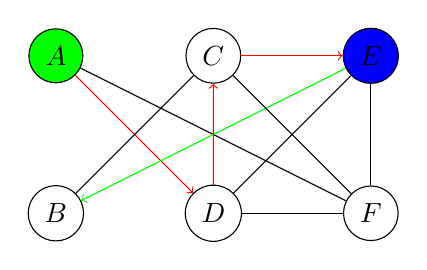
\begin{tikzpicture}
            \node[draw, circle, fill=green] (A) at (0,0) {$A$};
            \node[draw, circle] (B) at (0,-2) {$B$};
            \node[draw, circle] (C) at (2,0) {$C$};
            \node[draw, circle] (D) at (2,-2) {$D$};
            \node[draw, circle, fill=blue] (E) at (4,0) {$E$};
            \node[draw, circle] (F) at (4,-2) {$F$};

            \draw[->, red] (A) -- (D);
            \draw (A) -- (F);
            \draw (B) -- (C);
            \draw[->, green] (E) -- (B);
            \draw[->, red] (D) -- (C);
            \draw (C) -- (F);
            \draw (D) -- (E);
            \draw (E) -- (F);
            \draw[->, red] (C) -- (E);
            \draw (F) -- (D);
        \end{tikzpicture}
    \end{center}
\end{frame}

\begin{frame}{Część 2 - Algorytm Fleury'ego: przykład}
    \begin{itemize}
        \item Jesteś w wierzchołku $B$. Umieść go na stosie.
        \item Wybierz krawędź wychodzącą z wierzchołka $B$, która nie jest mostem.
        \item Nie ma takiej krawędzi, jest tylko most do $C$. Nie mając wyboru, wybierz tę krawędź.
        \item Przejdź do wierzchołka $C$ i usuń krawędź z grafu.
        \item Stos: $A$, $D$, $C$, $E$, $B$
    \end{itemize}
    \begin{center}
        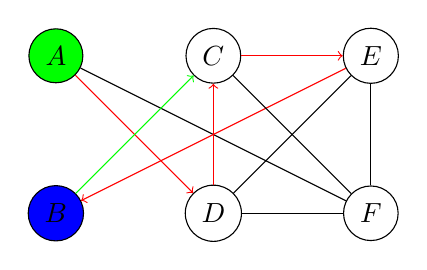
\begin{tikzpicture}
            \node[draw, circle, fill=green] (A) at (0,0) {$A$};
            \node[draw, circle, fill=blue] (B) at (0,-2) {$B$};
            \node[draw, circle] (C) at (2,0) {$C$};
            \node[draw, circle] (D) at (2,-2) {$D$};
            \node[draw, circle] (E) at (4,0) {$E$};
            \node[draw, circle] (F) at (4,-2) {$F$};

            \draw[->, red] (A) -- (D);
            \draw (A) -- (F);
            \draw[->, green] (B) -- (C);
            \draw[->, red] (E) -- (B);
            \draw[->, red] (D) -- (C);
            \draw (C) -- (F);
            \draw (D) -- (E);
            \draw (E) -- (F);
            \draw[->, red] (C) -- (E);
            \draw (F) -- (D);
        \end{tikzpicture}
    \end{center}
\end{frame}

\begin{frame}{Część 2 - Algorytm Fleury'ego: przykład}
    \begin{itemize}
        \item Jesteś w wierzchołku $C$. Umieść go na stosie.
        \item Wybierz krawędź wychodzącą z wierzchołka $C$, która nie jest mostem.
        \item Nie ma takich krawędzi, jest tylko most do $F$. Nie mając wyboru, wybierz tę krawędź.
        \item Przejdź do wierzchołka $F$ i usuń krawędź z grafu.
        \item Stos: $A$, $D$, $C$, $E$, $B$, $C$
    \end{itemize}
    \begin{center}
        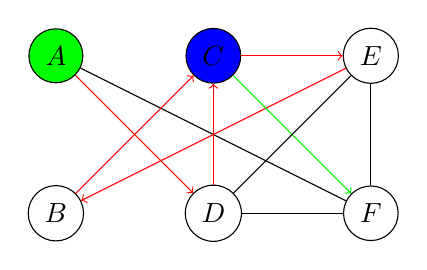
\begin{tikzpicture}
            \node[draw, circle, fill=green] (A) at (0,0) {$A$};
            \node[draw, circle] (B) at (0,-2) {$B$};
            \node[draw, circle, fill=blue] (C) at (2,0) {$C$};
            \node[draw, circle] (D) at (2,-2) {$D$};
            \node[draw, circle] (E) at (4,0) {$E$};
            \node[draw, circle] (F) at (4,-2) {$F$};

            \draw[->, red] (A) -- (D);
            \draw (A) -- (F);
            \draw[->, red] (B) -- (C);
            \draw[->, red] (E) -- (B);
            \draw[->, red] (D) -- (C);
            \draw[->, green] (C) -- (F);
            \draw (D) -- (E);
            \draw (E) -- (F);
            \draw[->, red] (C) -- (E);
            \draw (F) -- (D);
        \end{tikzpicture}
    \end{center}
\end{frame}

\begin{frame}{Część 2 - Algorytm Fleury'ego: przykład}
    \begin{itemize}
        \item Jesteś w wierzchołku $F$. Umieść go na stosie.
        \item Wybierz krawędź wychodzącą z wierzchołka $F$, która nie jest mostem, na przykład krawędź do $E$.
        \item Przejdź do wierzchołka $E$ i usuń krawędź z grafu.
        \item Stos: $A$, $D$, $C$, $E$, $B$, $C$, $F$
    \end{itemize}
    \begin{center}
        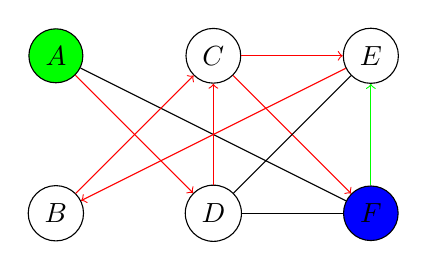
\begin{tikzpicture}
            \node[draw, circle, fill=green] (A) at (0,0) {$A$};
            \node[draw, circle] (B) at (0,-2) {$B$};
            \node[draw, circle] (C) at (2,0) {$C$};
            \node[draw, circle] (D) at (2,-2) {$D$};
            \node[draw, circle] (E) at (4,0) {$E$};
            \node[draw, circle, fill=blue] (F) at (4,-2) {$F$};

            \draw[->, red] (A) -- (D);
            \draw (A) -- (F);
            \draw[->, red] (B) -- (C);
            \draw[->, red] (E) -- (B);
            \draw[->, red] (D) -- (C);
            \draw[->, red] (C) -- (F);
            \draw (D) -- (E);
            \draw[->, green] (F) -- (E);
            \draw[->, red] (C) -- (E);
            \draw (F) -- (D);
        \end{tikzpicture}
    \end{center}
\end{frame}

\begin{frame}{Część 2 - Algorytm Fleury'ego: przykład}
    \begin{itemize}
        \item Jesteś w wierzchołku $E$. Umieść go na stosie.
        \item Wybierz krawędź wychodzącą z wierzchołka $E$, która nie jest mostem - została tylko krawędź do $D$.
        \item Przejdź do wierzchołka D i usuń krawędź z grafu.
        \item Stos: $A$, $D$, $C$, $E$, $B$, $C$, $F$, $E$
    \end{itemize}
    \begin{center}
        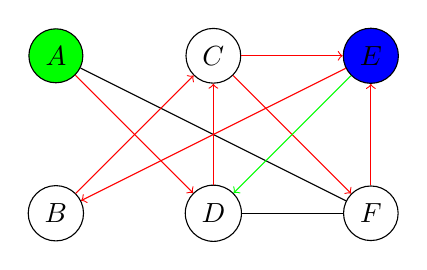
\begin{tikzpicture}
            \node[draw, circle, fill=green] (A) at (0,0) {$A$};
            \node[draw, circle] (B) at (0,-2) {$B$};
            \node[draw, circle] (C) at (2,0) {$C$};
            \node[draw, circle] (D) at (2,-2) {$D$};
            \node[draw, circle, fill=blue] (E) at (4,0) {$E$};
            \node[draw, circle] (F) at (4,-2) {$F$};

            \draw[->, red] (A) -- (D);
            \draw (A) -- (F);
            \draw[->, red] (B) -- (C);
            \draw[->, red] (E) -- (B);
            \draw[->, red] (D) -- (C);
            \draw[->, red] (C) -- (F);
            \draw[->, green] (E) -- (D);
            \draw[->, red] (F) -- (E);
            \draw[->, red] (C) -- (E);
            \draw (F) -- (D);
        \end{tikzpicture}
    \end{center}
\end{frame}

\begin{frame}{Część 2 - Algorytm Fleury'ego: przykład}
    \begin{itemize}
        \item Jesteś w wierzchołku $D$. Umieść go na stosie.
        \item Wybierz krawędź wychodzącą z wierzchołka $D$, która nie jest mostem - została tylko krawędź do $F$.
        \item Przejdź do wierzchołka $F$ i usuń krawędź z grafu.
        \item Stos: $A$, $D$, $C$, $E$, $B$, $C$, $F$, $E$, $D$
    \end{itemize}
    \begin{center}
        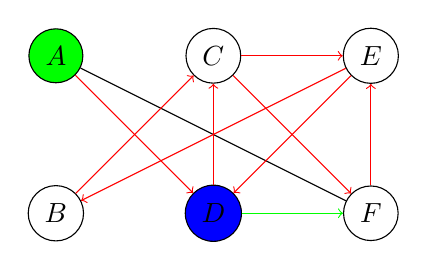
\begin{tikzpicture}
            \node[draw, circle, fill=green] (A) at (0,0) {$A$};
            \node[draw, circle] (B) at (0,-2) {$B$};
            \node[draw, circle] (C) at (2,0) {$C$};
            \node[draw, circle, fill=blue] (D) at (2,-2) {$D$};
            \node[draw, circle] (E) at (4,0) {$E$};
            \node[draw, circle] (F) at (4,-2) {$F$};

            \draw[->, red] (A) -- (D);
            \draw (A) -- (F);
            \draw[->, red] (B) -- (C);
            \draw[->, red] (E) -- (B);
            \draw[->, red] (D) -- (C);
            \draw[->, red] (C) -- (F);
            \draw[->, red] (E) -- (D);
            \draw[->, red] (F) -- (E);
            \draw[->, red] (C) -- (E);
            \draw[->, green] (D) -- (F);
        \end{tikzpicture}
    \end{center}
\end{frame}

\begin{frame}{Część 2 - Algorytm Fleury'ego: przykład}
    \begin{itemize}
        \item Jesteś w wierzchołku $F$. Umieść go na stosie.
        \item Wybierz krawędź wychodzącą z wierzchołka $F$, która nie jest mostem - została tylko krawędź do $A$.
        \item Przejdź do wierzchołka $A$ i usuń krawędź z grafu.
        \item Stos: $A$, $D$, $C$, $E$, $B$, $C$, $F$, $E$, $D$, $F$
    \end{itemize}
    \begin{center}
        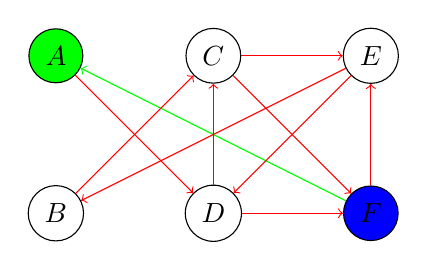
\begin{tikzpicture}
            \node[draw, circle, fill=green] (A) at (0,0) {$A$};
            \node[draw, circle] (B) at (0,-2) {$B$};
            \node[draw, circle] (C) at (2,0) {$C$};
            \node[draw, circle] (D) at (2,-2) {$D$};
            \node[draw, circle] (E) at (4,0) {$E$};
            \node[draw, circle, fill=blue] (F) at (4,-2) {$F$};

            \draw[->, red] (A) -- (D);
            \draw[->, green] (F) -- (A);
            \draw[->, red] (B) -- (C);
            \draw[->, red] (E) -- (B);
            \draw[->, red] (D) -- (C);
            \draw[->, red] (C) -- (F);
            \draw[->, red] (E) -- (D);
            \draw[->, red] (F) -- (E);
            \draw[->, red] (C) -- (E);
            \draw[->, red] (D) -- (F);
        \end{tikzpicture}
    \end{center}
\end{frame}


\begin{frame}{Część 2 - Algorytm Fleury'ego: przykład}
    \begin{itemize}
        \item Jesteś w wierzchołku $A$. Umieść go na stosie.
        \item Wybierz krawędź wychodzącą z wierzchołka $A$. Nie ma takiej krawędzi.
        \item Sprawdź, czy zostały nieodwiedzone krawędzie. Nie - stos w odwrotnej kolejności tworzy szukany cykl Eulera.
        \item Stos: $A$, $D$, $C$, $E$, $B$, $C$, $F$, $E$, $D$, $F$, $A$
    \end{itemize}
    \begin{center}
        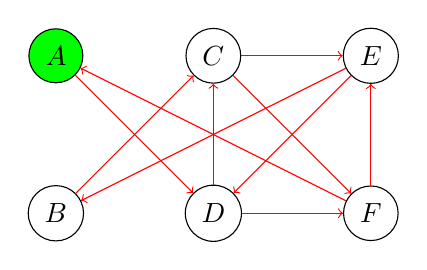
\begin{tikzpicture}
            \node[draw, circle, fill=green] (A) at (0,0) {$A$};
            \node[draw, circle] (B) at (0,-2) {$B$};
            \node[draw, circle] (C) at (2,0) {$C$};
            \node[draw, circle] (D) at (2,-2) {$D$};
            \node[draw, circle] (E) at (4,0) {$E$};
            \node[draw, circle] (F) at (4,-2) {$F$};

            \draw[->, red] (A) -- (D);
            \draw[->, red] (F) -- (A);
            \draw[->, red] (B) -- (C);
            \draw[->, red] (E) -- (B);
            \draw[->, red] (D) -- (C);
            \draw[->, red] (C) -- (F);
            \draw[->, red] (E) -- (D);
            \draw[->, red] (F) -- (E);
            \draw[->, red] (C) -- (E);
            \draw[->, red] (D) -- (F);
        \end{tikzpicture}
    \end{center}
\end{frame}

\begin{frame}{Część 2 - Algorytm Hierholzera}
    \begin{block}{Algorytm Hierholzera}
        \begin{itemize}
            \item Algorytm Hierholzera jest używany do znalezienia cyklu eulera w grafie.
            \item Jest on wydajniejszą, a jednocześnie bardziej skomplikowaną alternatywą dla algorytmu Fleury'ego.
            \item Nazwa algorytmu pochodzi od niemieckiego matematyka Carla Hierholzera, który pracował nad tym problemem w latach 1873-1874.
            \item Zauważył on, że cykl Eulera jest sumą cykli prostych o rozłącznych krawędziach.
            \item Algorytm pozwala znajdować cykle Eulera w grafach skierowanych i nieskierowanych.
            \item Złożoność: $\mathcal{O}(|E|)$
        \end{itemize}
    \end{block}
\end{frame}
    
\begin{frame}{Część 2 - działanie algorytmu Hierholzera}
    \begin{enumerate}
        \item Rozpocznij od wybranego wierzchołka w grafie eulerowskim.
        \item Wybierz dowolną krawędź wychodzącą z bieżącego wierzchołka i dodaj ją do ścieżki.
        \item Usuń wybraną krawędź z grafu.
        \item Przejdź do wierzchołka, do którego prowadzi wybrana krawędź.
        \item Jeśli bieżący wierzchołek ma jeszcze dostępne krawędzie, wróć do kroku 2 i kontynuuj.
        \item Jeśli bieżący wierzchołek nie ma już dostępnych krawędzi i istnieją inne wierzchołki na ścieżce, znajdź ostatni wierzchołek na ścieżce, który ma dostępne krawędzie i wróć do niego.
        \item Powtarzaj kroki 2-6, aż nie zostaną odwiedzone wszystkie krawędzie i utworzony zostanie cykl eulera.
    \end{enumerate}
\end{frame}

\begin{frame}{Część 2 - algorytm Hierholzera: przykład}
    \begin{itemize}
        \item Rozważmy poniższy nieważony, nieskierowany graf eulerowski.
    \end{itemize}
    \begin{center}
        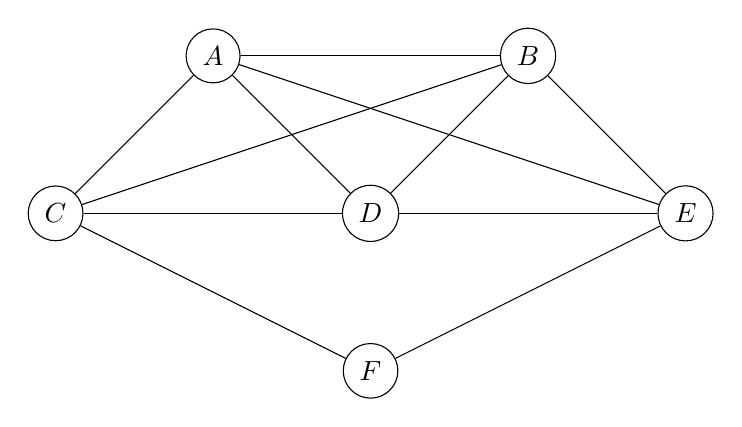
\begin{tikzpicture}
            \node[draw, circle] (A) at (-2,2) {$A$};
            \node[draw, circle] (B) at (2,2) {$B$};
            \node[draw, circle] (C) at (-4,0) {$C$};
            \node[draw, circle] (D) at (0,0) {$D$};
            \node[draw, circle] (E) at (4,0) {$E$};
            \node[draw, circle] (F) at (0,-2) {$F$};

            \draw (A) -- (B);
            \draw (A) -- (C);
            \draw (A) -- (D);
            \draw (A) -- (E);
            \draw (B) -- (C);
            \draw (B) -- (D);
            \draw (B) -- (E);
            \draw (C) -- (D);
            \draw (C) -- (F);
            \draw (D) -- (E);
            \draw (E) -- (F);
        \end{tikzpicture}
    \end{center}
\end{frame}

\begin{frame}{Część 2 - Algorytm Hierholzera: przykład}
    \begin{itemize}
        \item Wybierz wierzchołek startowy np. $A$ - oznaczony kolorem zielonym.
        \item Znajdujemy cykl prosty rozpoczynający się w tym wierzchołku.
        \item Cykl umieszczamy na liście, a z grafu usuwamy wszystkie krawędzie tego cyklu.
        \item C: $A$ $B$ $C$ $A$
    \end{itemize}
    \begin{center}
        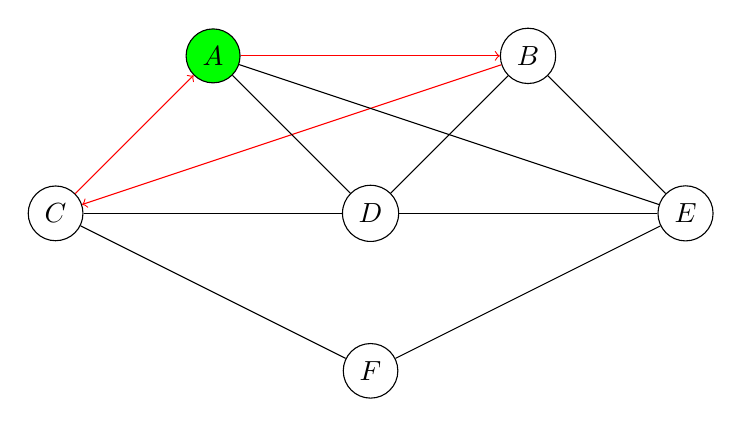
\begin{tikzpicture}
            \node[draw, circle, fill=green] (A) at (-2,2) {$A$};
            \node[draw, circle] (B) at (2,2) {$B$};
            \node[draw, circle] (C) at (-4,0) {$C$};
            \node[draw, circle] (D) at (0,0) {$D$};
            \node[draw, circle] (E) at (4,0) {$E$};
            \node[draw, circle] (F) at (0,-2) {$F$};

            \draw (A)[->, red] -- (B);
            \draw (C)[->, red] -- (A);
            \draw (B)[->, red] -- (C);
            \draw (A) -- (D);
            \draw (A) -- (E);
            \draw (B) -- (D);
            \draw (B) -- (E);
            \draw (C) -- (D);
            \draw (C) -- (F);
            \draw (D) -- (E);
            \draw (E) -- (F);
        \end{tikzpicture}
    \end{center}
\end{frame}


\begin{frame}{Część 2 - Algorytm Hierholzera: przykład}
    \begin{itemize}
        \item Przeglądając listę cyklu C wybieramy wierzchołek, który wciąż posiada incydentne krawędzie np. $A$.
        \item Znajdujemy cykl prosty rozpoczynający się w tym wierzchołku.
        \item Cykl umieszczamy na liście, a z grafu usuwamy wszystkie krawędzie tego cyklu.
        \item C: [$A$] $B$ $C$ $A$
        \item C: [$A$] $D$ $B$ $F$ $A$ $B$ $C$ $A$
    \end{itemize}
    \begin{center}
        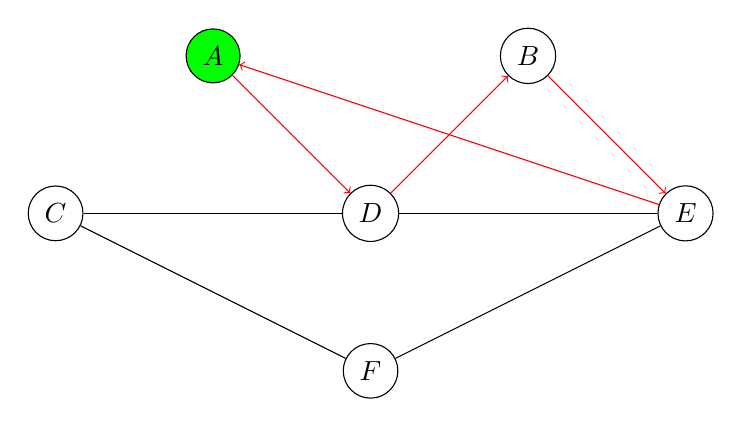
\begin{tikzpicture}
            \node[draw, circle, fill=green] (A) at (-2,2) {$A$};
            \node[draw, circle] (B) at (2,2) {$B$};
            \node[draw, circle] (C) at (-4,0) {$C$};
            \node[draw, circle] (D) at (0,0) {$D$};
            \node[draw, circle] (E) at (4,0) {$E$};
            \node[draw, circle] (F) at (0,-2) {$F$};

            \draw (A)[->, red] -- (D);
            \draw (E)[->, red] -- (A);
            \draw (D)[->, red] -- (B);
            \draw (B)[->, red] -- (E);
            \draw (C) -- (D);
            \draw (C) -- (F);
            \draw (D) -- (E);
            \draw (E) -- (F);
        \end{tikzpicture}
    \end{center}
\end{frame}

\begin{frame}{Część 2 - Algorytm Hierholzera: przykład}
    \begin{itemize}
        \item Przeglądając listę cyklu C wybieramy wierzchołek, który wciąż posiada incydentne krawędzie np. $D$.
        \item Znajdujemy cykl prosty rozpoczynający się w tym wierzchołku.
        \item Cykl umieszczamy na liście, a z grafu usuwamy wszystkie krawędzie tego cyklu.
        \item C: $A$ [$D$] $B$ $F$ $A$ $B$ $C$ $A$
        \item C: $A$ [$D$] $C$ $F$ $E$ $D$ $B$ $F$ $A$ $B$ $C$ $A$
    \end{itemize}
    \begin{center}
        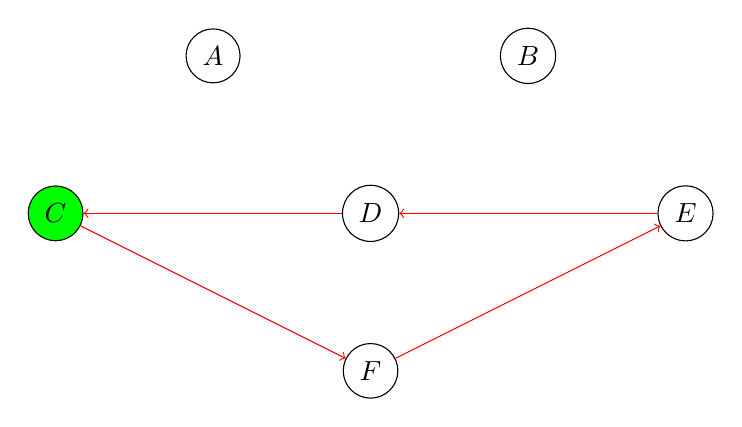
\begin{tikzpicture}
            \node[draw, circle] (A) at (-2,2) {$A$};
            \node[draw, circle] (B) at (2,2) {$B$};
            \node[draw, circle, fill=green] (C) at (-4,0) {$C$};
            \node[draw, circle] (D) at (0,0) {$D$};
            \node[draw, circle] (E) at (4,0) {$E$};
            \node[draw, circle] (F) at (0,-2) {$F$};

            \draw (D)[->, red] -- (C);
            \draw (C)[->, red] -- (F);
            \draw (E)[->, red] -- (D);
            \draw (F)[->, red] -- (E);
        \end{tikzpicture}
    \end{center}
\end{frame}

\begin{frame}{Część 2 - Algorytm Hierholzera: przykład}
    \begin{itemize}
        \item Lista C nie zawiera już wierzchołków o niezerowym stopniu.
        \item Lista C zawiera cykl Eulera.
        \item C: $A$ $D$ $C$ $F$ $E$ $D$ $B$ $F$ $A$ $B$ $C$ $A$
    \end{itemize}
    \begin{center}
        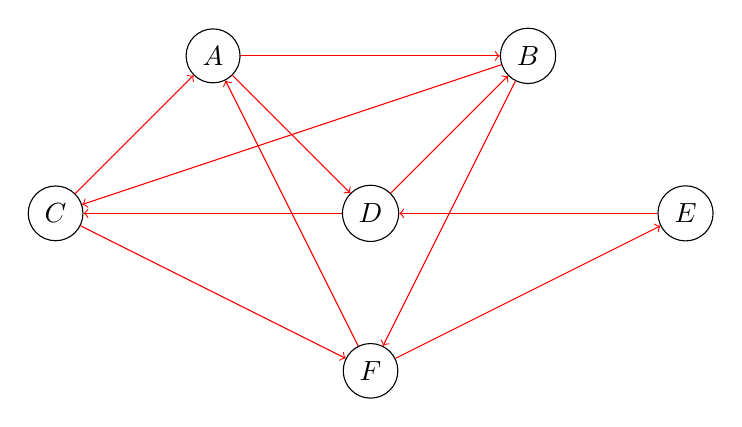
\begin{tikzpicture}
            \node[draw, circle] (A) at (-2,2) {$A$};
            \node[draw, circle] (B) at (2,2) {$B$};
            \node[draw, circle] (C) at (-4,0) {$C$};
            \node[draw, circle] (D) at (0,0) {$D$};
            \node[draw, circle] (E) at (4,0) {$E$};
            \node[draw, circle] (F) at (0,-2) {$F$};

            \draw(A)[->, red] -- (D);
            \draw(D)[->, red] -- (C);
            \draw(C)[->, red] -- (F);
            \draw(F)[->, red] -- (E);
            \draw(E)[->, red] -- (D);
            \draw(D)[->, red] -- (B);
            \draw(B)[->, red] -- (F);
            \draw(F)[->, red] -- (A);
            \draw(A)[->, red] -- (B);
            \draw(B)[->, red] -- (C);
            \draw(C)[->, red] -- (A);
        \end{tikzpicture}
    \end{center}
\end{frame}

\begin{frame}{Część 3 - Grafy półeulerowskie, nieważone}
    \begin{block}{}
        \begin{itemize}
            \item W grafach tych, w porównaniu do ulerowskich wystarczy dodać krawędź łączącą wierzchołki o nieparzystym stopniu.
            \item Otrzymujemy w ten sposób graf eulerowski, w którym możemy znaleźć cykl korzystając z wcześniej wspomnianych algorytmów.
            \item Po znalezieniu cyklu, usuwamy uprzednio dodaną krawędź otrzymując ścieżkę Eulera.
            \item Aby otrzymać ścieżkę zamkniętą, można znaleźć najkrótszą ścieżkę łączącą dwa wierzchołki nieparzystego stopnia (np. algorytm Dijkstry ($\mathcal{O}({E} \cdot {\log V})$))
        \end{itemize}
    \end{block}
\end{frame}

\begin{frame}{Część 4 - Grafy eulerowskie, ważone}
    \begin{block}{}
        \begin{itemize}
            \item W grafach tych, w porównaniu do wersji nieważonej, wystarczy zsumować wagę wszystkich krawędzi.
            \item Graf eulerowski posiada tylko jeden cykl Eulera.
            \item Korzystamy z wcześniej omówionych algorytmów.
        \end{itemize}
    \end{block}
\end{frame}

\begin{frame}{Część 5 - Grafy półeulerowskie, ważone}
    \begin{block}{}
        \begin{itemize}
            \item W grafach tych, w porównaniu do wersji nieważonej, wystarczy zsumować wagę wszystkich krawędzi.
            \item Dołożona krawędź może mieć dowolną wagę - przy jej usunięciu waga zostanie odjęta od sumy.
            \item Graf eulerowski posiada tylko jeden cykl Eulera.
            \item Korzystamy z wcześniej omówionych algorytmów.
            \item Aby otrzymać ścieżkę zamkniętą, można znaleźć najkrótszą ścieżkę łączącą dwa wierzchołki nieparzystego stopnia (np. algorytm Dijkstry ($\mathcal{O}({E} \cdot {\log V})$))
        \end{itemize}
    \end{block}
\end{frame}

\begin{frame}{Część 6 - Algorytm ogólny - graf spójny}
    \begin{block}{Algorytm ogólny}
        \begin{itemize}
            \item Jeśli graf zawiera więcej niż dwa wierzchołki o nieparzystych stopniach, problem staje się trudny obliczeniowo.
            \item Lemat o uściskach dłoni -  liczba wierzchołków o nieparzystych stopniach w grafie spójnym jest zawsze liczbą parzystą.
            \item Wierzchołki możemy połączyć w pary za pomocą znalezionych ścieżek.
            \item \textbf{Problem:} Suma wag użytych do połączeń ścieżek winna być minimalna, ponieważ będą one dublowane celem uzyskania parzystego stopnia wierzchołków.
            \item Problem znajdowania skojarzeń par wierzchołków o minimalnych wagach krawędzi rozwiązuje \textbf{algorytm Edmondsa} o złożoności $\mathcal{O}(|V|^{3})$.
        \end{itemize}
    \end{block}
\end{frame}

\begin{frame}{Część 6 - Algorytm ogólny - graf spójny}
    \begin{block}{Algorytm ogólny}
        \begin{enumerate}
            \item Sprawdź czy graf jest spójny - jeżeli nie zakończ.
            \item Wyszukaj w grafie wszystkie wierzchołki o nieparzystych stopniach.
            \item Jeżeli liczba ta jest równa 0, idź do kroku 7.
            \item Wyznacz za pomocą np. algorytmu Dijkstry ($\mathcal{O}({E} \cdot {\log V})$) lub Bellmana-Ford'a ($\mathcal{O}(|E| \cdot |V|)$) najkrótsze ścieżki łączące ze sobą wszystkie znalezione wierzchołki o nieparzystych stopniach.
            \item Wyszukaj doskonałe skojarzenie tych wierzchołków w pary o najmniejszej sumie wag (algorytm Edmondsa).
            \item Krawędzie wchodzące w skład wyznaczonych ścieżek zdubluj w grafie wejściowym.
            \item Wyznacz w powstałym multigrafie cykl Eulera i wyprowadź wynik.
        \end{enumerate}
    \end{block}
\end{frame}

\begin{frame}{Część 7 - zastosowania problemu chińskiego listonosza}
    \begin{block}{Zastosowania}
        Problem Chińskiego Listonosza ma zastosowanie w dziedzinach, w których konieczne jest znalezienie
        optymalnej trasy lub cykly, który odwiedza wszystkie krawędzie z minimalnym kosztem.
    \end{block}
\end{frame}

\begin{frame}{Część 7 - zastosowania problemu chińskiego listonosza}
    \begin{block}{Automatyczna eksploracja sieci połączeń - roboty indeksujące}
        Wyszukiwarki takie jak Google, Bing, Yahoo korzystają z robotów indeksujących do skanowania i indeksowania
        treści stron internetowych. \\\textbf{Problem:} Jak odwiedzić jak najwięcej stron minimalnym kosztem?
    \end{block}
    \begin{block}{Automatyczna eksploracja sieci połączeń - optymalizacja dostępu do treści}
        Aplikacje, które pobierają treści z wielu miejsc w internecie. \\\textbf{Problem:} Jak zoptymalizować kolejność pobierania zasobów minimalizując koszty transferu danych?
    \end{block}
\end{frame}

\begin{frame}{Bibliografia}
    \begin{thebibliography}{99}
            \bibitem{1} Materiały wykładowe - Teoria grafów i sieci - prof. dr. hab. M.Kubale
            \bibitem{2} Materiały lekcyjne - mgr Jerzy Wałaszek - I LO im. Kazimierza Brodzińskiego w Tarnowie \\\url{https://eduinf.waw.pl/inf/alg/001_search/0122.php}
            \bibitem{3} Algorytm Edmonds'a - Luis Goddyn \\\url{https://eduinf.waw.pl/inf/alg/001_search/data/edmonds.pdf}
            \bibitem{4} M.Szachniuk, A.Świercz Politechnika Poznańska \\\url{http://www.cs.put.poznan.pl/mszachniuk/mszachniuk_files/lab_aisd/Szachniuk-ASD-t4.pdf}
    \end{thebibliography}
\end{frame}

\end{document}